\chapter{Experiments}

In this chapter we present our results and compare them to existing approaches.

\section{Datasets and metrics}

Dummy text.

\subsection{Datasets}

To get the Wikipedia pages, we use the dump from \emph{01 October 2012} that
has only the latest revision for each article \todo{Footnote for where to get
it}. The dump version we use should not impact the results considerably. We
happen to use the 2012 version just because was easily available at the time.
For this Wikipedia version we extract articles corresponding to a category (or
multiple categories recursively) recursively -- we parse the category graph
downwards starting from the given \emph{root} category. After extracting the
articles we keep only non-stub, human-written articles and we exclude all meta
pages. For more information about the extraction process see
\todo{coverage.WikiToPlainText section}.

We tested our approach on the following recursively extracted categories:
\begin{description}
  \item[Classical composers] Contains \(7246\) articles representing all
  classical music composers -- this is our biggest category apart from using all
  Wikipedia;
  \item[Game \acl{AI}] Contains \(471\) articles about the use
  of \ac{AI} in games (for example, chess, go, video games);
  \item[Machine learning] Contains \(735\) articles about the machine learning
  field;
  \item[Vectors] Contains \(341\) articles about mathematical vectors -- this
  our most abstract category;
\end{description}
and merges of them:
\begin{description}
  \item[Last 3] Contains the \(1547\) articles of the last three categories
  described above (Game \ac{AI}, Machine learning, Vectors);
  \item[All 4] Contains the \(8793\) articles of all above categories
  (Composers, Game \ac{AI}, Machine learning, Vectors).
\end{description}
For the final results we used the \textbf{2012 Wikipedia} which has a total of
\(1.3\) million \todo{double check this number} non-stub, human-written
articles (excluding meta pages).

In addition to the Wikipedia subset, we use the \emph{\acf{NIPS}} dataset --
contains \(1955\) papers -- and the \emph{\acf{ACL}} dataset -- contains
\(18041\) papers -- to test our baseline implementations against their authors
\cite{sipos2012temporal}.

\subsection{Metrics}

We have looked to find metrics suitable to our task of finding the most
important, valuable Wikipedia articles, but we could not find a reliable method
that also fits well to our use case.
Some of the possible metrics are:
\begin{description}
  \item[Number of inlinks] This metric is similar to the use of \emph{number of
  citations} presented in \cite{sipos2012temporal}, but extended to web pages.
  While it does not have the same limitations as citations, it is hard to
  guarantee its validity \todo{citation needed}.
  \item[PageRank] A common way to extend the use of just inlinks which solves a
  lot of the problems with inlinks.
  \todo{citation needed}.
  \item[Condensed Wikipedia] Count the number of selected documents that appear
  in a condensed Wikipedia version used in education or in emph{Wikispeedia}
  \todo{citation needed}.
\end{description}

For the purposes of this thesis we use \emph{number of inlinks} as we view
Wikipedia as a non-competitive environment (different from the game between
search engines and malevolent web masters).

\subsection{Graphs and tables}
\todo{Explain the format.}

\section{Baselines}

Dummy text. \todo{Explain ALL the results!}

\subsection{Random}

Dummy text.
\begin{figure}
  \centering
  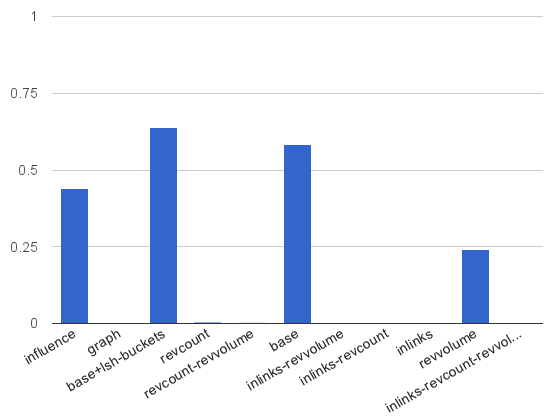
\includegraphics[width=0.9\textwidth,natwidth=555,natheight=419]{images/rand-mean.png}
  \caption{The score of the \emph{random selected} sets as given by the other
  submodular functions}
  \label{img:rand-mean}
\end{figure}

\subsection{Word coverage}

Dummy text.
\begin{figure}
  \centering
  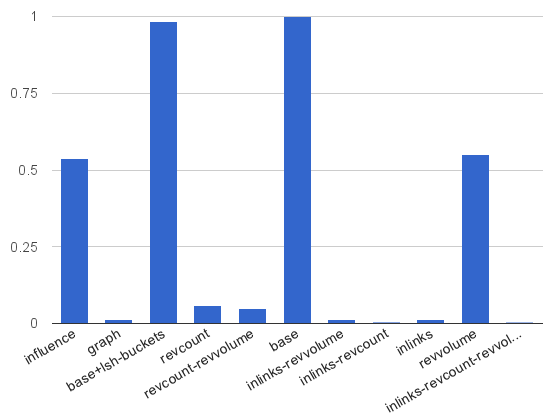
\includegraphics[width=0.9\textwidth,natwidth=555,natheight=419]{images/wc.png}
  \caption{The score of the \emph{word coverage} set as given by the other
  submodular functions}
  \label{img:wc}
\end{figure}

\begin{table}
    \begin{tabular}{lll}
    1  & History of Western civilization                  & 115   \\
    2  & Stephen Tompkinson                               & 78    \\
    3  & Timeline of United States inventions (1890–1945) & 381   \\
    4  & November 2013                                    & 102   \\
    5  & Education in the United States                   & 1098  \\
    6  & American Civil War bibliography                  & 320   \\
    7  & Races of the Mass Effect universe                & 42    \\
    8  & October 2011 in sports                           & 98    \\
    9  & Prince (musician)                                & 2458  \\
    10 & Stowe House                                      & 109   \\
    11 & Outline of science                               & 12    \\
    12 & 2000 New Year Honours                            & 77    \\
    13 & Seasons in Scottish football                     & 856   \\
    14 & Lists of state leaders by year                   & 2563  \\
    15 & The Idler (1758–1760)                            & 32    \\
    16 & National Football League                         & 22939 \\
    17 & Disasters of the Century                         & 8     \\
    18 & Sustainable Services                             & 1     \\
    19 & Australian of the Year                           & 232   \\
    20 & Largest organisms                                & 41    \\
    \end{tabular}
    \caption {Top 20 articles selected by the \emph{word coverage} function.}
\end{table}

\subsection{Document influence}

Dummy text.
\begin{figure}
  \centering
  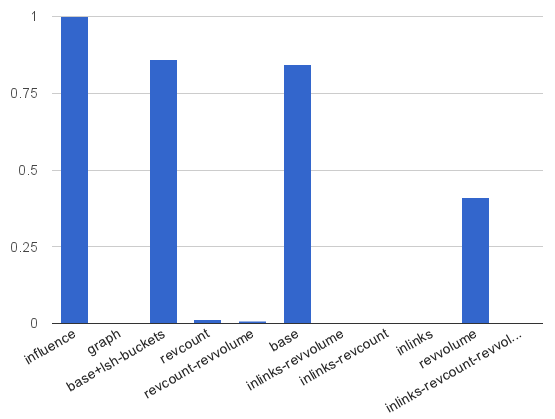
\includegraphics[width=0.9\textwidth,natwidth=555,natheight=419]{images/infl.png}
  \caption{The scores of the \emph{document influence} set as given by the
  other submodular functions}
  \label{img:infl}
\end{figure}

\section{Graph coverage}

Dummy text.
\begin{figure}
  \centering
  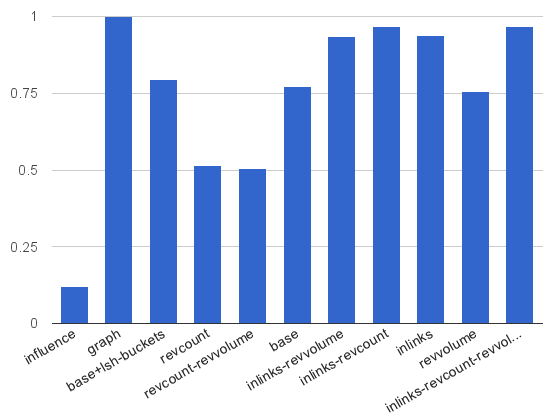
\includegraphics[width=0.9\textwidth,natwidth=555,natheight=419]{images/graph.png}
  \caption{The scores of the \emph{graph coverage} set as given by the other
  submodular functions}
  \label{img:graph}
\end{figure}

\section{\ac{LSH} buckets}

Dummy text.
\begin{figure}
  \centering
  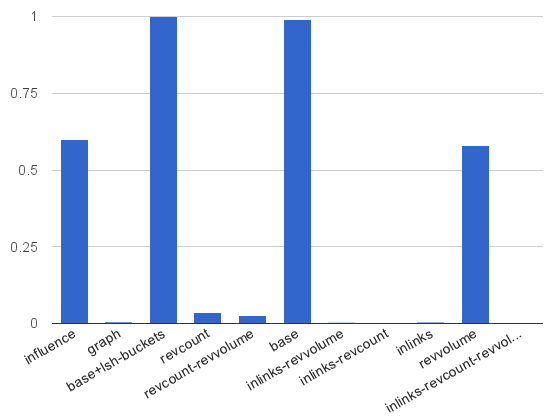
\includegraphics[width=0.9\textwidth,natwidth=555,natheight=419]{images/wc+lsh.png}
  \caption{The scores of the set selected by \emph{\ac{LSH} buckets} linearly
  combined with \emph{word coverage} as given by the other submodular
  functions}
  \label{img:wc+lsh}
\end{figure}

\section{Beyond word coverage}

Dummy text.
\begin{figure}
  \centering
  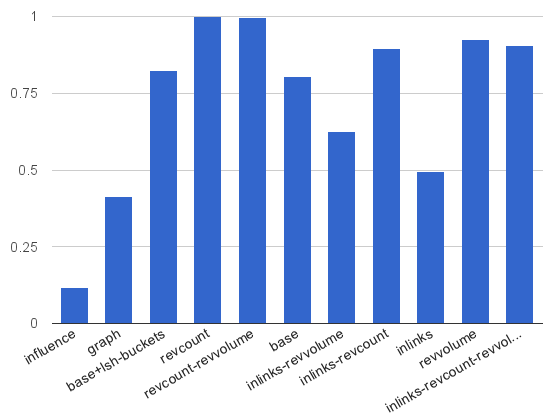
\includegraphics[width=0.9\textwidth,natwidth=555,natheight=419]{images/rc.png}
  \caption{The scores of the \emph{tf-idf -- revisions count} set as given by
  the other submodular functions}
  \label{img:rc}
\end{figure}

\begin{figure}
  \centering
  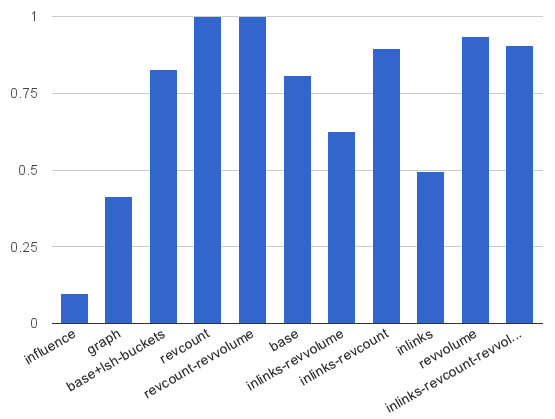
\includegraphics[width=0.9\textwidth,natwidth=555,natheight=419]{images/rc-rv.png}
  \caption{The scores of the \emph{tf-idf -- revisions count -- revisions
  volume} set as given by the other submodular functions}
  \label{img:rc-rv}
\end{figure}

\begin{figure}
  \centering
  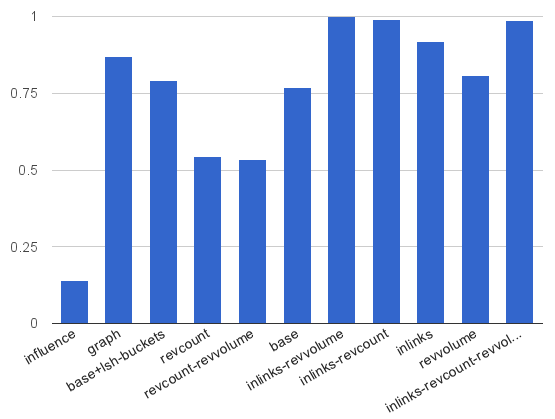
\includegraphics[width=0.9\textwidth,natwidth=555,natheight=419]{images/inl-rv.png}
  \caption{The scores of the \emph{tf-idf -- inlinks count -- revisions volume}
  set as given by the other submodular functions}
  \label{img:inl-rv}
\end{figure}

\begin{figure}
  \centering
  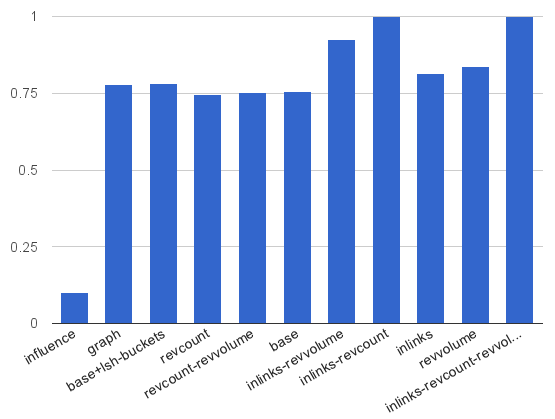
\includegraphics[width=0.9\textwidth,natwidth=555,natheight=419]{images/inl-rc.png}
  \caption{The scores of the \emph{tf-idf -- inlinks count -- revisions count}
  set as given by the other submodular functions}
  \label{img:inl-rc}
\end{figure}

\begin{figure}
  \centering
  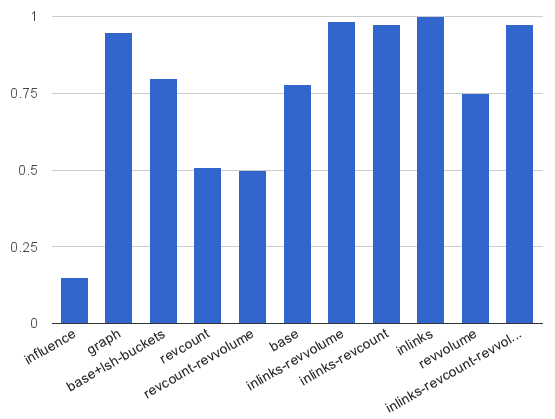
\includegraphics[width=0.9\textwidth,natwidth=555,natheight=419]{images/inl.png}
  \caption{The scores of the \emph{tf-idf -- inlinks count} set as given by the
  other submodular functions}
  \label{img:inl}
\end{figure}

\begin{figure}
  \centering
  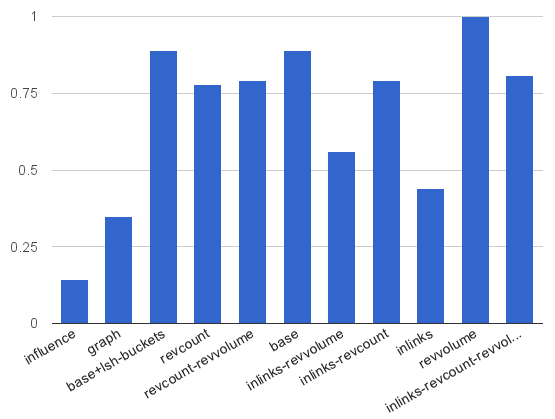
\includegraphics[width=0.9\textwidth,natwidth=555,natheight=419]{images/rv.png}
  \caption{The scores of the \emph{tf-idf -- revisions volume} set as given by
  the other submodular functions}
  \label{img:rv}
\end{figure}

\begin{figure}
  \centering
  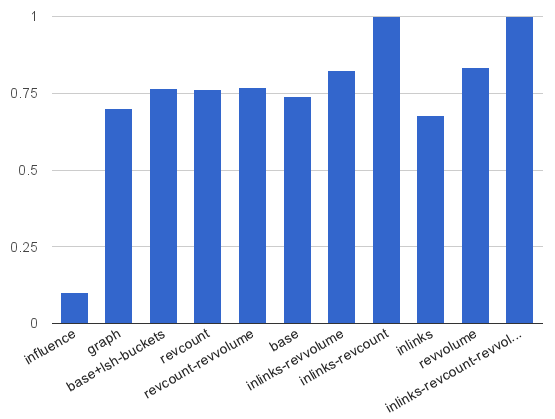
\includegraphics[width=0.9\textwidth,natwidth=555,natheight=419]{images/inl-rc-rv.png}
  \caption{The scores of the \emph{tf-idf -- inlinks count -- revisions count
  -- revisions volume} set as given by the other submodular functions}
  \label{img:}
\end{figure}

\section{Running time}

Dummy text.

